% !TEX root = ../thesis.tex
\chapter{The state of the art}
%\chapter{Etsi nfv}
\label{chap:State of the Art}
In the following sections a brief description of ETSI NFV main concept and architecture will be given in order to better understand the problem and the implemented solutions proposed in this thesis.

\section{The ETSI}
The European Telecommunications Standard Institute (ETSI) is an institution that produces globally-applicable standards for Information and Communications Technologies (ICTs). It spaces from fixed to mobile, radio, aeronautical, broadcast and Internet technologies and is officially recognized by the European Union as an European Standards Organization. ETSI is an independent, not-for-profit association whose more than 700 member companies and organizations located on over sixty countries across five continents worldwide, determine its work programme and participate directly in its work. In November 2012 seven of the world's leading telecoms network operators selected ETSI to be the home of the Industry Specification Group (ISG) for Network Function Virtualization (NFV). Now, almost two years later, a large community of experts are working intensely to develop the required standards for Network Functions Virtualization as well as sharing their experiences of NFV development and earlier implementation. The membership of ISG NFV has grown to over 230 individual companies including 37 of the world's major service providers as well as representatives from both telecoms and IT vendors.

\section{Objectives}
From a high point of view, the objectives that the ETSI NFV group established:
\begin{itemize}
	\item Improve capital efficiencies compared with the one obtained by using dedicated hardware implementations. This is achieved by using commercial-off-the-shelf (COTS) hardware (i.e. general purpose servers and storage devices) to provide Network Functions (NFs) through software virtualization techniques. Because of their nature, these functions are commonly referred as Virtualized Network Functions (VNFs). Also the sharing of hardware and reducing the number of different physical server architectures in a network contribute to this objective in the sense of allowing larger stock orders and hardware re-usage.
	\item Improve flexibility in assigning VNFs to hardware. This aids both scalability and largely separates functionality from location, which allows software to be located in the most appropriate places referred to from now on as NFV Infrastructure Points of Presence (NFVI-PoPs) for example at customers' premises, at network exchange points, in central offices, data-centers, etc. These features enable time of day reuse, support for test of alpha/beta and production versions, enhance resilience through virtualization, and facilitate resource sharing.
	\item Rapid service innovation through automated software-based deployment.
	\item Improve operational efficiency resulting from common automation and operating procedures.
	\item Reduce power usage, achieved by migrating workloads and powering down unused hardware (i.e. an idling server can be shout down).
	\item Provide Standardized and open interfaces between virtualized network functions, the infrastructure and associated management entities so that such decoupled elements can be provided by different vendors.
\end{itemize}

\section{High-level NFV framework}
Network Functions Virtualization envisages the implementation of NFs as software-only entities that run over the NFV Infrastructure (NFVI). Figure \ref{fig:etsi_hl_nfv_framework} illustrates the high-level NFV framework. As such, three main working domains are identified in network function virtualization:
\begin{itemize}
	\item NFV Infrastructure (NFVI), including the diversity of physical resources and the way that these can be virtualized. NFVI supports the execution of the VNFs.

	\item Virtualized Network Function in the sense of the software implementation of a NF which is capable of running over the NFVI.
	
	\item NFV Management and Orchestration, which covers the arrangement and life-cycle governance of physical and/or software resources that support the infrastructure virtualization other than the life-cycle management of VNFs. This point focuses on all virtualization-specific management tasks necessary in the NFV framework.
\end{itemize}
\begin{figure}[h]
	\centering
	% left bottom right top
	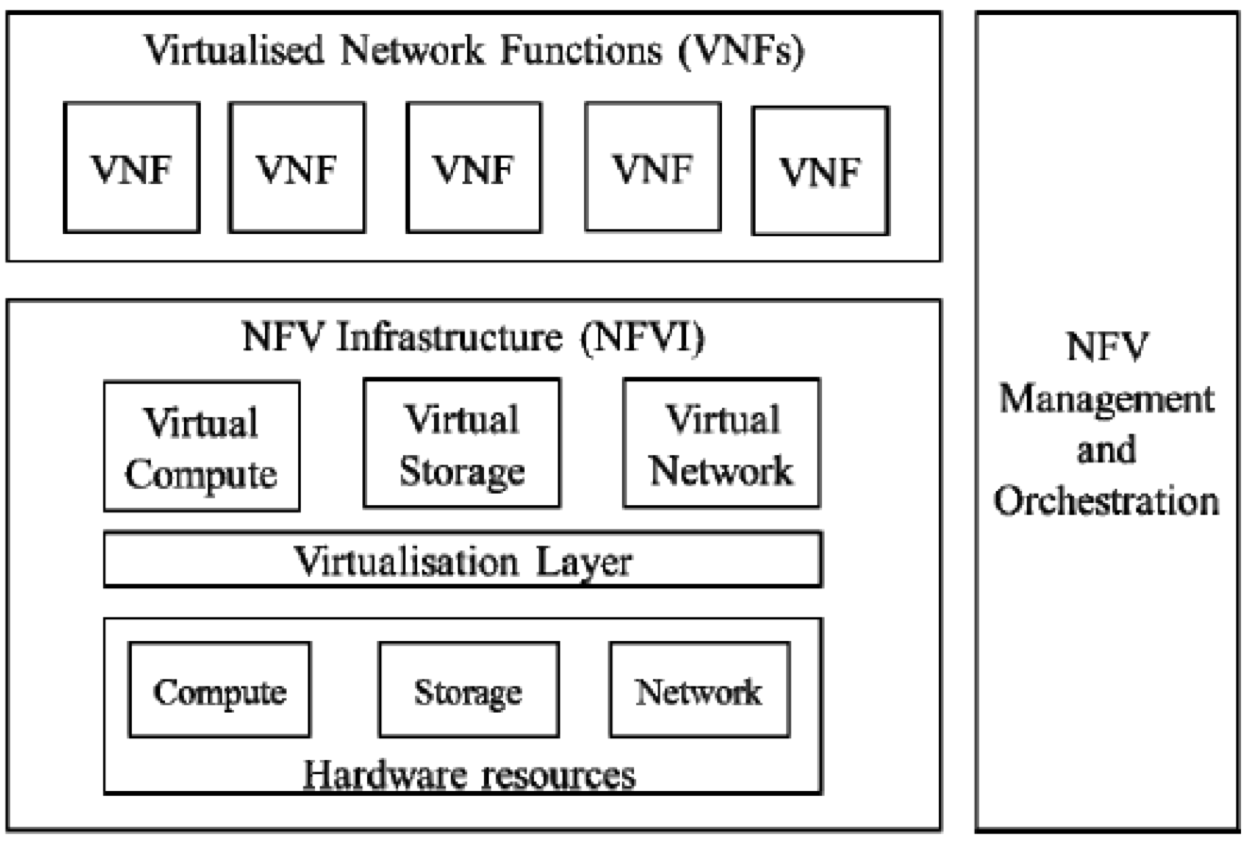
\includegraphics[clip= true, width= \columnwidth]{images/ETSI_Architectural_framework.png}
	\caption{ETSI - High-level NFV framework architecture}
	\label{fig:etsi_hl_nfv_framework}
\end{figure}

The NFV framework enables dynamic construction and management of VNF instances and the relationships between them in term of data, control, management, dependencies and other attributes. To this end there are at least three architectural views of VNFs that are centered around different points of view and contexts of a VNF. These perspectives include:
\begin{itemize}
	\item A virtualization deployment/on-boarding angle where the context can be a VM.
	\item A vendor-developed software package perspective where the context can be several inter-connected VMs and a deployment template that describes their attributes.
	\item An operator point of view where the context can be the operation and management of a VNF received in the form of a vendor software package.
\end{itemize}


Within each of just mentioned contexts , at least the following relations exist between VNFs:
\begin{itemize}
	\item A VNF Set covers the case where the connectivity between VNFs is not specified.
	\item A VNF Forwarding Graph (VNF-FG) covers the case where network connectivity does matter, for instance a chain of VNFs in a web server tier (e.g. firewall, NAT, load balancer)	
\end{itemize}

\section{Network services in NFV}
An end-to-end network service (e.g. mobile voice/data, Internet access, a virtual private network) can be described by an NF Forwarding Graph of interconnected Network Functions (NFs) and end points. The termination points and the NFs of the network service are represented as nodes and correspond to devices, applications, and/or physical server applications. An NF Forwarding Graph can have network function nodes connected by logical links that can be unidirectional, bidirectional, multicast and/or broadcast.
In figure \ref{fig:end2end_network_service} is shown an example of an end-to-end network service and the different layers that are involved in its virtualization process. The depicted example offers a clear view of the abstraction (upper part) and how it is remapped to the underlaying physical infrastructure (NFVI). It consists in an end-to-end network service composed by five general purpose VNFs and two termination (end) points. The decoupling of hardware and software in NFV is realized by a virtualization layer. This layer abstracts hardware resources of the NFV Infrastructure.

\begin{figure}[h]
	\centering
	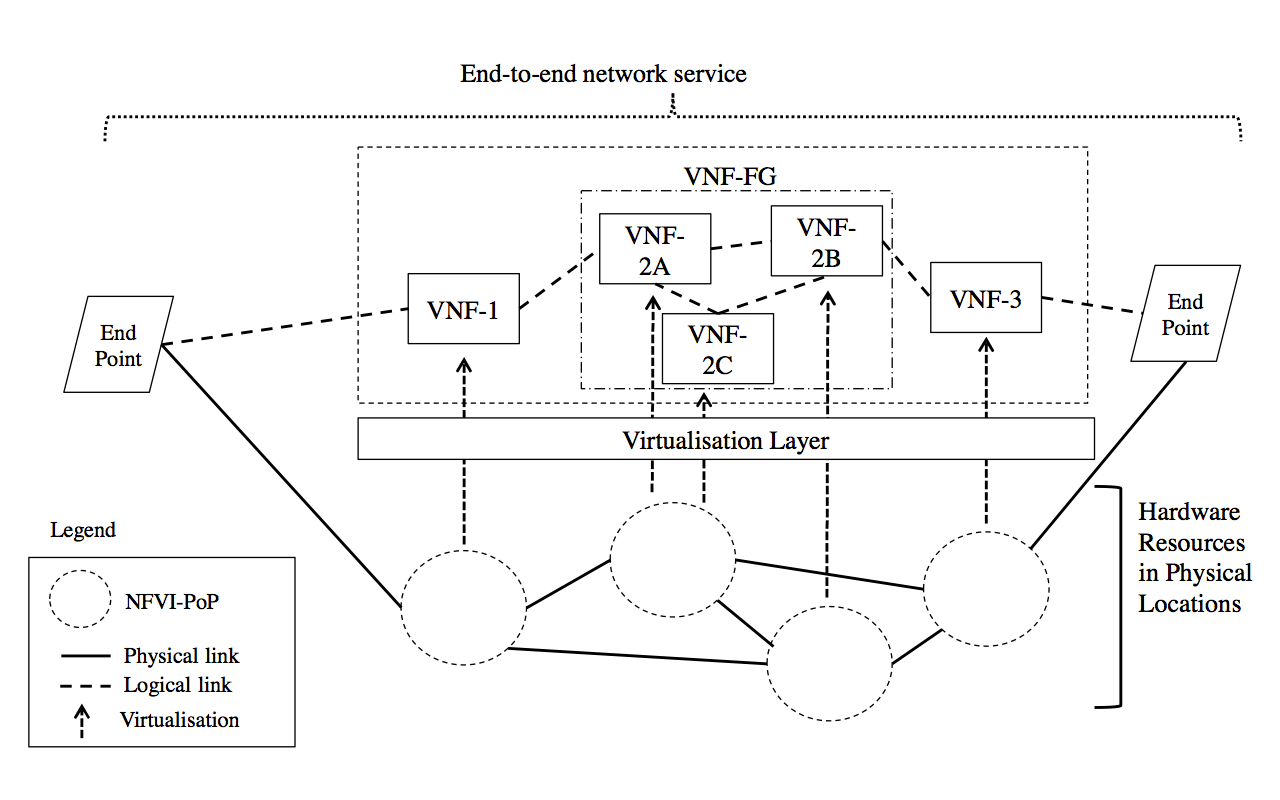
\includegraphics[clip= true, width= \columnwidth]{images/network_service.png}
	\caption{ETSI - end-to-end network service with VNFs and nested forwarding graphs example}
	\label{fig:end2end_network_service}
\end{figure}

\section{Architecture of NFV}
The NFV architectural framework identifies functional blocks and the main reference points between such blocks. The functional blocks are:
\begin{itemize}
	\item Virtualized Network Function (VNF).
	\item Element Management System (EMS).
	\item NFV Infrastructure, including:
	\item Hardware and virtualized resources, and
	\item Virtualization Layer.
	\item Virtualized Infrastructure Manager(s).
	\item Orchestrator.
	\item VNF Manager(s).
	\item Service, VNF and Infrastructure Description.
	\item Operations and Business Support Systems (OSS/BSS).
\end{itemize}

Figure \ref{fig:etsi_detailed_nfv_framework} shows the NFV architectural framework depicting the functional blocks and reference points in the NFV framework. The illustrated architectural framework focuses on the functionalities necessary for the virtualization and the consequent operation of operators' networks. It does not specify which network functions should be virtualized, as that is solely a decision of the owner of the network.
\begin{figure}[h]
	\centering
	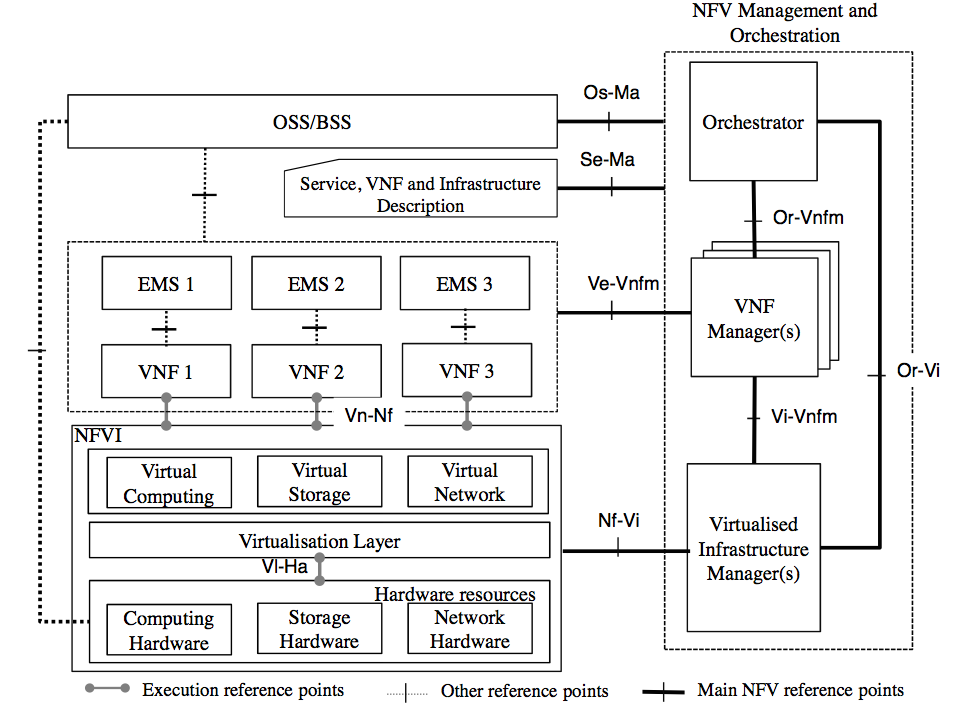
\includegraphics[clip= true, width= \columnwidth]{images/architettura_etsi.png}
	\caption{ETSI - Detailed NFV framework architecture}
	\label{fig:etsi_detailed_nfv_framework}
\end{figure}

\subsection{Functional blocks}
A functional block defined by ETSI is the basic unit of a system and consists of:
\begin{itemize}
	\item A set of input interfaces.
	\item A state.
	\item A transfer function.
	\item A set of output interfaces.
\end{itemize}
For sake of clarity, a view of a functional block is given in figure \ref{fig:functional_block}.
\begin{figure}[h]
	\centering
	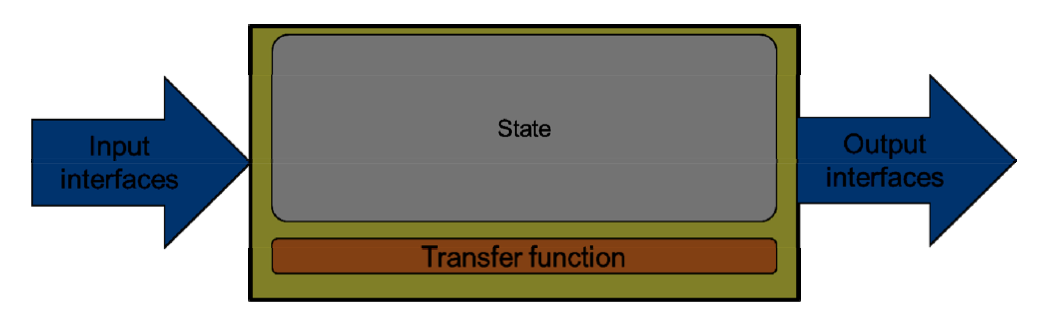
\includegraphics[clip= true, width= \columnwidth]{images/functional_block.png}
		\caption{ETSI - The fundamentals of a functional block}
	\label{fig:functional_block}
\end{figure}
A fundamental property of functional blocks is the complete and formal separation of the static from the dynamic. Using a more IT oriented terminology, the input, output, and internal (i.e. state) data structures and all the methods (i.e. the transfer function) are static. They shall not change. Only the values given as input parameters - and therefore the outputs - can change; these values are the only things labeled as dynamic.
Functional blocks are linked together following two fundamental rules:
\begin{itemize}
	\item They can be interconnected, by connecting an output interface of one functional block with the input interface of another functional block.
	\item When a number of functional blocks are interconnected together forming a topology, some input and some output interfaces may remain disconnected. In this case the resulting topology is, in turn, considered as a functional block itself in which the inputs and outputs are the endpoints that remained unlinked in the previous passage. The new obtained functional block follows the very same rules as a standard one.
\end{itemize}

\section{Templates}

ETSI introduces five descriptor for deployment and lifecycle management of VNF and NS:
\begin{itemize}
	\item Network Service Descriptor (NSD)
	\item VNF Descriptor (VNFD)
	\item VNF Forwarding Graph Descriptor (VNFFGD)
	\item Virtual Link Descriptor (VLD) 
	\item Physical Network Function Descriptor (PNFD) 
\end{itemize}

A Network Service Descriptor is a deployment template for a Network Service referencing all other descriptors which, in turn, describe components that are part of that Network Service. A VNF Descriptor is a deployment template which describes a VNF in terms of its deployment and operational behaviour requirements. It is primarily used by the VNF Manager in the process of VNF instantiation and lifecycle management of a VNF instance. The information provided in the VNFD is also used by the NFV Orchestrator to manage and orchestrate Network Services and virtualised resources on the NFV Infrastructure. The VNFD olso contain information for Management and orchestration layer (MANO) functional blocks that allow to establish appropriate Virtual Links with NFVI between its VNF Component (VNFC) instances or between a VNF instance and the endpoint interface to the other Network Functions. A VNF Forwarding Graph Descriptor (VNFFGD) is a deployment template which describes a topology of the Network Service or a portion of the Network Service, by referencing  VNFs and Phisical NFs (PNF) and Virtual Links that connect them. Essentially defines the path  that traffic must follow between VNFs. A Virtual Link Descriptor is a deployment template which describes the resource requirements that are needed for a link between VNFs, PNFs and endpoints of the Network Service, which could be met by various link options that are available in the NFVI. The NFV Orchestrator can select an option following consultation of the VNFFG to determine the appropriate NFVI to be used based on functional (e.g., dual separate paths for resilience) and other needs (e.g., geography and regulatory requirements). 
A Physical Network Function Descriptor (PNFD) describes the connectivity, Interface and KPIs requirements of virtual Links to an attached Physical Network Function.
At last there is the Physical Network Function Descriptor that delineates the connectivity, the interface and \servecitazione{key performance indicator} requirements of virtual links that are terminated on one side by a Physical Network Function(PNF); this flexibility is needed if hardware devices are incorporated in a Network Service, for example to facilitate the transition torward a fully virtualized environment.

In addition of containing descriptors, NSD also contains connection points and, optionally, dependencies between VNFs. By connection point is meant an information element representing the virtual and/or physical interface that offers connectivity between instances of NS, VNF, VNFC, PNF and a VL. Examples of virtual and physical interfaces are a virtual ports, a virtual NIC addresses, physical ports, physical NIC addresses or endpoints of an IP VPN.
The meaning of dependencies between VNFs is quickly explained via an example; let's say that for some reasons a function must exist and be connected to the service before another can be initiated/deployed and connected.

